\chapter{Implementación de la Solución}

La implementación de la solución cuenta con distintos módulos que usan distintas
tecnologías y potencialmente distintos lenguajes. Primero, para los módulos del
sistema se detallan las tecnologías escogidas, y luego se presentan las
interfaces creadas para los distintos actores (perfiles de usuario) del proceso.

\section{Tecnologías Escogidas para la Implementación}

En este apartado se describen los componentes críticos del sistema implementado,
y cuáles fueron las tecnologías usadas para tal propósito en cada caso. Antes de
eso, en todo caso, vale la pena explicar los requerimientos de implementación de
este sistema. Para ello, hay que tener muy claro qué capacidades tiene
actualmente la aplicación, cuál es su perspectiva de evolución a futuro, y cómo
será la operación de la misma. Estos tres puntos son claves para tomar cualquier
decisión con respecto a las tecnologías que se escojan para implementar el
sistema.

Primero que todo, este sistema muestra que se puede obtener datos desde UCampus
y usarlos para automatizar de forma interna el proceso de evaluación de las
postulaciones. Luego, el futuro de este sistema puede tomar dos rumbos: 1) los
datos se extraerán desde una API que exponga UCampus, o 2) la plataforma UCampus
estandariza el formulario de postulación a todos los programas de la Facultad
(hoy en día dicho formulario no está estandarizado). 

La segunda alternativa es poco viable en el corto plazo, pues requiere que todos
los programas de la Facultad se pongan de acuerdo acerca de qué información debe
aportar el postulante a la hora de postular a uno de ellos. Esto parece ser
difícil de alcanzar, pues muchos de estos programas tienen naturaleza distinta
(algunos tienen un perfil profesional y otros científico), y distintos niveles
de exigencia (por ejemplo, para magíster y doctorado).

Considerando estos aspectos, el sistema de evaluación de postulaciones debe
estar preparado para el futuro de varias formas: 

\begin{itemize}
\item Debe ser extensible, en el sentido de que debe permitir cambiar el método
de extracción de datos de las postulaciones.
\item Debe ser altamente mantenible, pues hay componentes que su actual
implementación depende de componentes o condiciones externas, que podrían
cambiar en un futuro inmediato. A pesar de eso el sistema debería poder
adaptarse en forma rápida para seguir brindando el servicio.
\item La operación de este sistema debe presentar la menor cantidad de
impedimentos, y bloqueos técnicos posibles, tanto para los desarrolladores como
para los administradores de sistemas.
\end{itemize}

A continuación se explican las tecnologías que se utilizaron para implementar
los macro-componentes de este sistema.

\subsection{Back-end}

El back-end es la piedra angular de esta aplicación. Dentro de él, funcionan el
scraper, la conexión a la base de datos y la disponibilización de los datos de
forma segura. Para implementar el back-end, la primera restricción es que
presenta, es que existen dos maneras viables para extraer los datos de las
postulaciones desde UCampus; cada una con su propio entorno de desarrollo. Una
de ellas usa Node.js, y otra está en Python.

Para tomar esta decisión, la Stack Overflow Developer Survey 2020 [10] reveló
que Python es el tercer lenguaje más amado por desarrolladores, sólo superado
por TypeScript y Rust. Python es además el lenguaje que más desarrolladores
buscan aprender.

A pesar de lo antes mencionado, sigue estando la opción de usar Puppeteer [3]
con TypeScript para implementar el back-end. Sin embargo, teniendo en cuenta el
perfil de los potenciales desarrolladores que tendrá el sistema, el uso de
Python parece ser la opción más apropiada para implementar el back-end del
sistema. Python es un lenguaje que cualquier estudiante de una Universidad
chilena conoce, al contrario de TypeScript, que si bien es un lenguaje con mucha
popularidad en la industria, no lo es tanto en el mundo académico.

Por las razones mencionadas anteriormente, el lenguaje escogido para escribir el
back-end es Python. Dado eso, queda por decidir cómo conectarse a la base de
datos, y cómo exponer los datos de las postulaciones de forma segura.


\subsubsection{Base de Datos}

La encuesta a desarrolladores mencionada anteriormente (de Stack Overflow)
mostró que PostgreSQL es la base de datos persistente más amada por estas
personas [10]. Le siguen, en orden, Elastic Search y MongoDB. Por otro lado,
PostgreSQL es la segunda base de datos que los desarrolladores buscan aprender,
sólo precedida por MongoDB.

La base de datos rankeada como \#1 en la encuesta es Redis [12]; sin embargo,
ésta no es una opción puesto que es una base de datos en memoria.

Con respecto a bases de datos SQL (PostgreSQL) y NoSQL (Elastic Search y
MongoDB), la naturaleza estructurada y relacional de los datos existentes hacen
que inclinarse por PostgreSQL sea una buena idea. Otra razón para ello es que
potenciales desarrolladores de este sistema muy probablemente no estarán muy
familiarizados con bases de datos NoSQL, pues son menos abordadas en cursos
bases de datos a nivel de pregrado. Por las razones anteriormente expuestas, se
decidió que los datos de este sistema se almacenen en una base de datos
PostgreSQL.

\subsubsection{Servidor HTTP}

Para el servidor HTTP se deben tomar en cuenta las siguiente consideraciones:

\begin{itemize}
\item Rendimiento (performance) del servidor, medido en cantidad de respuestas
por segundo.
\item Curva de aprendizaje para nuevos desarrolladores.
\end{itemize}

% ref tabla
Para evaluar el rendimiento potencial del servidor se analizó la información
disponible en the benchmarker [11], el cual consta de una serie de repositorios
dedicados a encontrar benchmarks de servidores HTTP en frameworks web. Para cada
framework se mide la cantidad de respuestas por segundo, según la cantidad de
threads concurrentes que intentan acceder al servidor. En la Tabla
\ref{table:frameworks} se muestra un resumen de los resultados obtenidos por los
frameworks más conocidos.

\begin{table}[!ht]
    \begin{center}
        \begin{tabular}{|l|l|l|r|r|r|}
            \hline
            \# & Lenguaje & Framework & Req/s (64) & Req/s (128) & Req/s (256) \\ \hline
            58 & python (3.9) & falcon (2.0) & 74.256,04 & 81.538,76 & 82.897,69 \\ \hline
            88 & python (3.9) & pyramid (2.0) & 51.298,30 & 56.850,32 & 57.128,55 \\ \hline
            100 & python (3.9) & asgineer (0.8) & 44.745,54 & 51.318,30 & 52.105,43 \\ \hline
            104 & python (3.9) & bottle (0.12) & 39.690,41 & 42.590,65 & 44.329,21 \\ \hline
            107 & python (3.9) & emmett (2.2) & 35.983,95 & 41.270,86 & 42.295,95 \\ \hline
            115 & python (3.9) & apidaora (0.28) & 34.119,60 & 38.263,87 & 38.707,73 \\ \hline
            116 & python (3.9) & hug (2.6) & 34.040,91 & 35.909,39 & 53.828,77 \\ \hline
            125 & python (3.9) & blacksheep (1.0) & 28.887,22 & 33.204,44 & 34.356,25 \\ \hline
            129 & python (3.9) & index.py (0.16) & 27.273,81 & 29.282,48 & 30.258,63 \\ \hline
            131 & python (3.9) & starlette (0.14) & 26.693,66 & 31.709,52 & 31.302,99 \\ \hline
            134 & python (3.9) & responder (2.0) & 26.092,65 & 31.092,58 & 32.175,53 \\ \hline
            135 & python (3.9) & clastic (199) & 25.651,88 & 28.936,99 & 28.781,05 \\ \hline
            136 & python (3.9) & sanic (21.3) & 25.446,08 & 28.833,98 & 29.194,50 \\ \hline
            145 & python (3.9) & molten (1.0) & 18.055,01 & 21.858,74 & 21.906,60 \\ \hline
            146 & python (3.9) & aiohttp (3.7) & 17.837,07 & 23.359,98 & 24.128,26 \\ \hline
            149 & python (3.9) & fastapi (0.63) & 16.701,72 & 22.402,72 & 22.042,29 \\ \hline
            164 & python (3.9) & flask (1.1) & 12.901,82 & 16.427,23 & 16.521,94 \\ \hline
            176 & python (3.9) & cherrypy (18.6) & 9.328,09 & 9.396,33 & 8.832,55 \\ \hline
            177 & python (3.9) & guillotina (6.2) & 9.152,33 & 8.843,65 & 8.742,31 \\ \hline
            181 & python (3.9) & quart (0.14) & 7.571,28 & 7.501,08 & 6.888,88 \\ \hline
            183 & python (3.9) & tonberry (0.2) & 7.363,12 & 6.948,61 & 6.344,40 \\ \hline
            191 & python (3.9) & django (3.1) & 5.918,73 & 6.572,13 & 6.150,29 \\ \hline
            193 & python (3.9) & tornado (6.1) & 5.722,03 & 5.728,67 & 5.624,07 \\ \hline
            210 & python (3.9) & masonite (3.0) & 2.485,30 & 2.477,63 & 2.477,29 \\ \hline
            217 & python (3.9) & cyclone (1.3) & 1.597,57 & 1.591,42 & 1.577,40 \\ \hline
            218 & python (3.9) & klein (20.6) & 1.501,11 & 1.538,24 & 1.513,71 \\ \hline
            220 & python (3.9) & nameko (2.13) & 1.213,25 & 1.164,90 & 1.142,60 \\ \hline
            222 & python (3.9) & django-ninja (0.11) & 1.065,37 & 1.478,17 & 1.496,42 \\ \hline
        \end{tabular}
    \end{center}
    \caption{Rendimiento de frameworks de Python. La primera columna indica la posición entre todos los frameworks testeados y desde la cuarta columna en adelante, el número representa la cantidad promedio de peticiones completadas por segundo para una cierta cantidad de clientes haciendo estas peticiones concurrentemente (el número indicado en paréntesis)}
    \label{table:frameworks}
\end{table}

La Tabla \ref{table:frameworks} muestra los resultados para herramientas python
que sirven para implementar el back-end del sistema. Las columnas de resultados
(que parten con \emph{Req/s}) indican cuántas peticiones por segundo puede
responder el servidor cuando hay una cierta cantidad de usuarios haciendo
peticiones de forma concurrente (el número entre los paréntesis).

En todo caso, hay que tener en cuenta que muchas de estas herramientas suelen
ser experimentales, y otras son tan minimales que no es viable su uso para
sistemas como el reportado en esta memoria.

Tomando en cuenta la popularidad de los paquetes, en término de cantidad de
estrellas en GitHub, los contendores son:

\begin{itemize}
    \item FastAPI (29.2k estrellas)
    \item Django (56.5k estrellas)
    \item Flask (54.4k estrellas)
\end{itemize}

FastAPI es el más nuevo de los tres y cuenta con soporte para asyncio [14], con
tutoriales cortos donde se explica la totalidad de sus capacidades. Django es el
más popular, con una gran cantidad de capacidades (tan grande de hecho, que no
se hacen necesarias todas ellas). Finalmente, Flask es prácticamente FastAPI,
pero sin soporte para asyncio, ni inyección de dependencias.

Considerando lo anterior, se decidió utilizar usar FastAPI tomando en cuenta
diversos aspectos:

\begin{itemize}
    \item Su gran popularidad pese a su poco tiempo de vida, comparado con Flask
    y Django.
    \item Soporta asyncio en forma nativa. El uso de asyncio hace que pueda
    manejar una mayor cantidad de peticiones por segundo.
    \item La barrera de entrada para usar este framework es mucho más pequeña
    que Django y es comparable a Flask. Por lo tanto, para el futuro de este
    proyecto, los nuevos desarrolladores no tendrán que entender la filosofía de
    un framework completo, como Django, sino que simplemente les bastará
    entender cómo funcionan los módulos de Python.
\end{itemize}

\subsection{Scraper}

Con respecto al scraper, ya se introdujo anteriormente las alternativas
evaluadas, estas eran: Puppeteer [3] y Selenium [4]. Al tomar en cuenta que
Selenium tiene bindings para Python, se hace evidente usarlo en vez de
Puppeteer. De nuevo, la mantenibilidad juega un rol importante en esta decisión.

\subsection{Deployment}

Para decidir cómo hacer el deployment de la aplicación, se tuvo en cuenta que el
sistema involucra, entre otros:

\begin{enumerate}
    \item Un módulo de scraping, que requiere ejecutables en el sistema
    operativo host.
    \item Una API.
    \item Ejecución continua del módulo de scraping.
\end{enumerate}

La instalación de un sistema con tales características no es trivial, pues no
sólo se necesita de las dependencias naturales de Python, sino además
componentes del sistema operativo para que funcione.

Para automatizar esa tarea y hacer el deployment de esta aplicación un proceso
confiable, Docker [13] es una herramienta que permite abstraer tales
restricciones y hace del deployment un proceso con bajo riesgo, pues no importa
el ambiente en el que se ejecuta el proyecto. En ese sentido, sólo basta que
funcione en Docker.

\subsection{Front-end}

Con respecto al front-end, los dos lenguajes más populares para implementar un
sitio web con sus interfaces son JavaScript y TypeScript. Existen otras opciones
que simplemente se descartan por baja popularidad, y por lo tanto, una
potencialmente baja capacidad para darle mantenimiento al sistema.

El Developer Survey 2020 de Stack Overflow [11] reveló que, de los frameworks
web más apreciados por los desarrolladores, React [15] está en la posición 2,
mientras que Vue.js [16] está en la posición 3; ambos superados por ASP.NET
Core, que se descarta usar en este proyecto simplemente porque requiere que el
servidor sea escrito en C\#, lenguaje que no es opción para este proyecto.

React [15] es el framework JavaScript más popular de front-end en el mercado, y
es elegido para el desarrollo de esta aplicación precisamente por eso. Como en
este proyecto se prioriza la mantenibilidad, React es probablemente la mejor
opción. Vue [16] es el segundo framework más popular. Sin embargo, al momento
del comienzo de la implementación de este sistema, Vue se encontraba en
transición entre la versión 2 a la 3. Por lo tanto, elegirlo habría implicado
trabajar con APIs inestables, o bien con APIs obsoletas. Por las razones
anteriormente expuestas, React es la opción elegida para este proyecto.

\section{Interfaces de Usuario}

En esta sección se presentan las principales interfaces de usuario del sistema.
El propósito de esto es ilustrar cómo se ayuda a los diferentes tipos de
usuario, a cumplir con sus tareas. Para evitar la sobre extensión del documento,
sólo se muestran las principales interfaces para cada usuario; es decir, sólo
aquellas que son críticas para el cumplimiento de las funciones asignadas a cada
rol.

En primer lugar se muestra la interfaz principal del sistema, a la cual se
accede luego del proceso de autenticación del usuario (Figura 8). En este caso
el usuario está logueado con el rol de asistente. Es importante aclarar que los
datos mostrados en estas interfaces son ficticios.

\begin{figure}[!ht]
    \begin{center}
        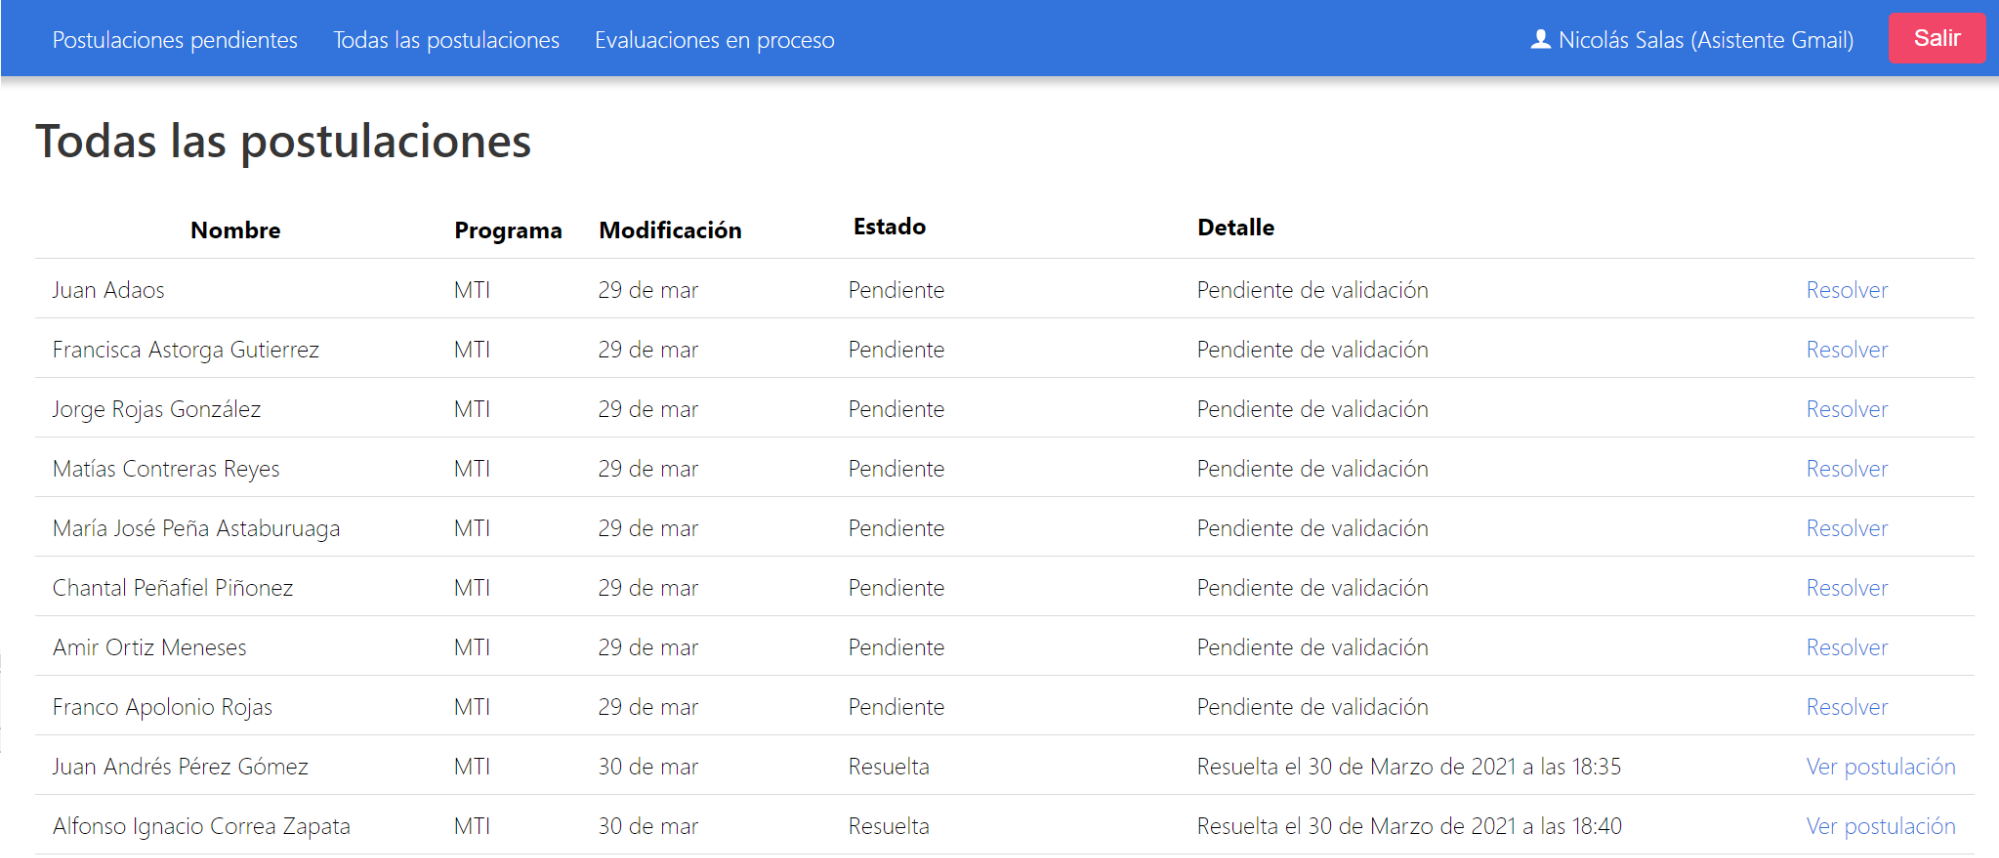
\includegraphics[scale=0.23]{imagenes/04-interfaz-principal.png}
    \end{center}
    \caption{Interfaz principal del sistema}
    \label{fig:interfaz-principal}
\end{figure}

El menú principal tiene tres opciones: postulaciones pendientes, todas las
postulaciones y postulaciones en proceso. La semántica de cada categoría varía
dependiendo del perfil de usuario que accede a la información. En el caso de la
Figura \ref{fig:interfaz-principal}, la información que se muestra corresponde a
“todas las postulaciones”, esto incluye las “pendientes de evaluación”, las “en
proceso” y las “resueltas”. A continuación se explican las principales
interfaces para cada rol.

\subsection{Interfaces de Usuario para el Asistente}

En el caso del usuario asistente, las postulaciones pendientes corresponden a
aquellas que aún no han sido mandadas a evaluar (Figura
\ref{fig:interfaz-pendientes}), probablemente porque aún no tienen todos los
documentos que se requiere para poder procesarlas. Para verificar esto, el
asistente debe clickear en el link “Resolver” de la postulación que quiere
revisar. Una vez hecho eso, accede a la postulación.

\begin{figure}[!ht]
    \begin{center}
        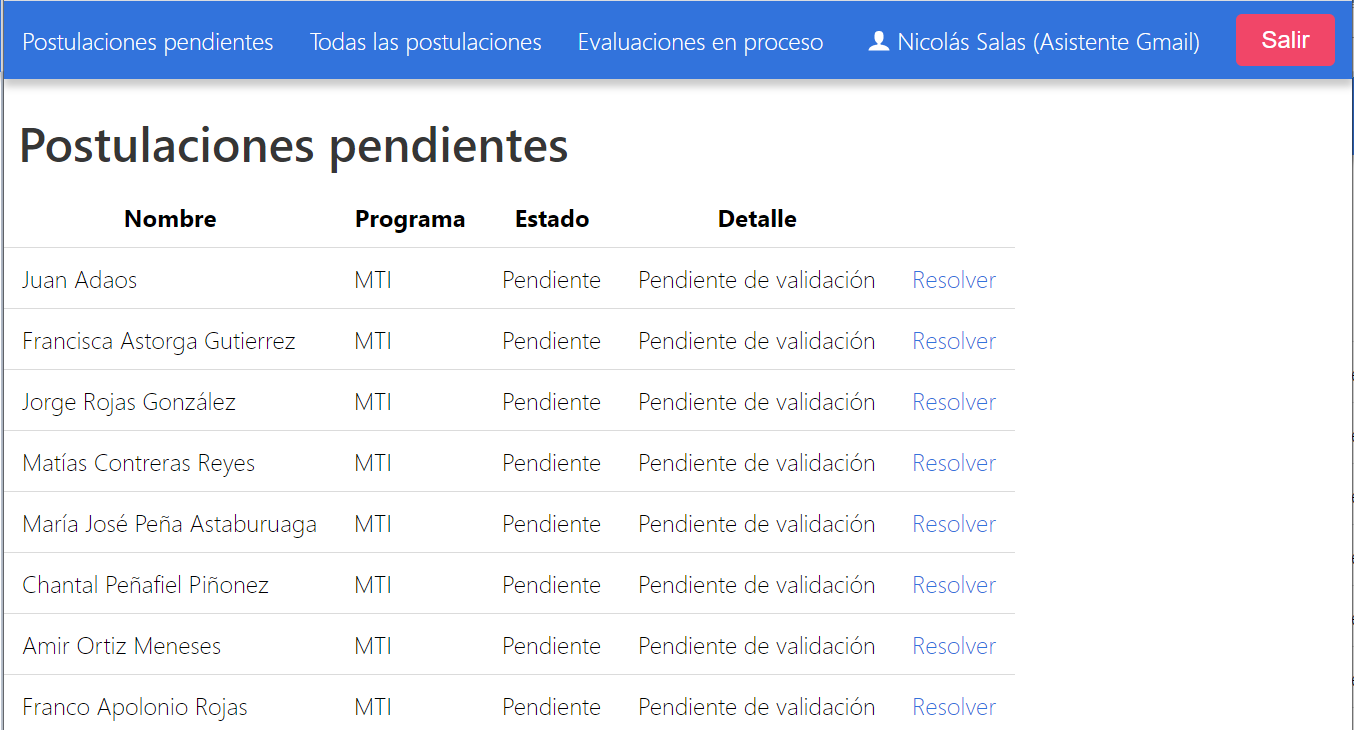
\includegraphics[scale=0.23]{imagenes/04-interfaz-pendientes.png}
    \end{center}
    \caption{Interfaz de postulaciones pendientes}
    \label{fig:interfaz-pendientes}
\end{figure}

La figura \ref{fig:formulario-antecedentes} muestra cómo se ven los datos de una
postulación para un usuario asistente. A la izquierda se muestran los datos
personales del postulante, que han sido ofuscados por temas de privacidad. En la
sección media de la interfaz se presentan los antecedentes académicos del
postulante, y a la derecha se encuentran los documentos requeridos por el
programa para que sea válida una postulación. Los documentos que han sido
subidos correctamente contienen un link; éste sirve para descargar dicho
documento y verificar que corresponde a lo requerido (por ejemplo, es un
Currículum Vitae). Los documentos que aparecen en rojo son aquellos que están
faltantes.

\begin{figure}[!ht]
    \begin{center}
        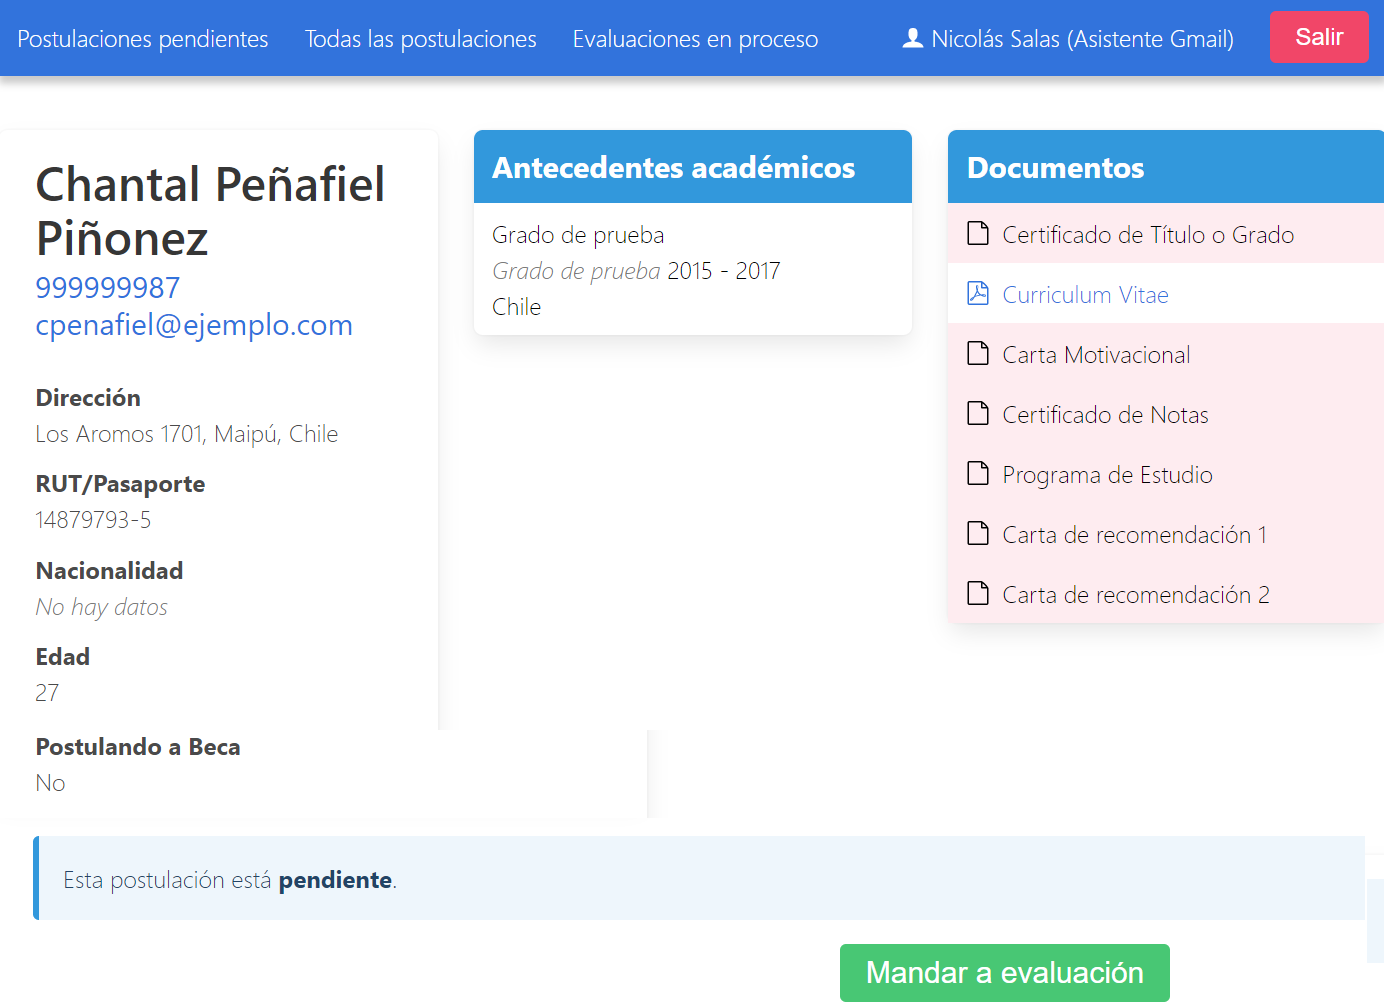
\includegraphics[scale=0.23]{imagenes/04-antecedentes-postulacion.png}
    \end{center}
    \caption{Formulario de antecedentes de la postulación}
    \label{fig:formulario-antecedentes}
\end{figure}

Aunque la postulación no tenga todos los datos que considera el formulario, ésta
se puede mandar a evaluar si tiene lo mínimo necesario. Para ello, al hacer
click en el botón “Mandar a Evaluación” (Figura
\ref{fig:formulario-antecedentes}), el sistema le informa al usuario el estado
de completitud de la postulación, y le pide confirmar la acción antes indicada
(Figura \ref{fig:confirmacion-evaluacion}).

\begin{figure}[!ht]
    \begin{center}
        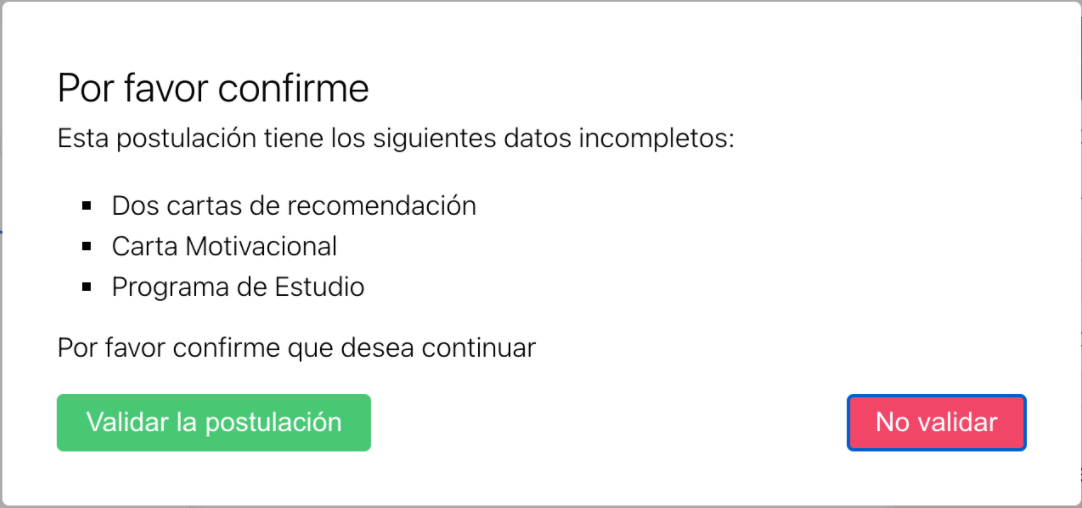
\includegraphics[scale=0.23]{imagenes/04-confirmacion-evaluacion.png}
    \end{center}
    \caption{Confirmación al mandar una postulación a evaluación}
    \label{fig:confirmacion-evaluacion}
\end{figure}

La opción “evaluaciones en proceso” para este perfil de usuario, al igual que
para el perfil coordinador, muestra las postulaciones que han sido enviadas a
evaluar y que aún no cuentan con una resolución por parte del coordinador. La
opción “todas las evaluaciones” muestra lo ya indicado en la figura
\ref{fig:interfaz-pendientes}.

\subsection{Interfaces de usuario para los Evaluadores}

Las interfaces de los usuarios evaluadores son similares a la de los usuarios
asistentes en términos de estructura e información mostrada. Sin embargo, los
evaluadores sólo pueden ver la información de las postulaciones asignadas a
ellos, mientras que los asistentes pueden ver todas las postulaciones.

Otra diferencia radica en la semántica de la opción de menú “evaluaciones
pendientes”, que en el caso de los evaluadores corresponde a las postulaciones
asignadas a ellos, pero sobre las cuales aún no emiten un juicio de aceptación o
rechazo.

Una tercera diferencia corresponde a que este perfil de usuario puede evaluar
una postulación, y para ello debe completar el formulario que se muestra en la
figura \ref{fig:formulario-evaluacion}. Los campos del formulario completo se
muestran en el Anexo B.

\begin{figure}[!ht]
    \begin{center}
        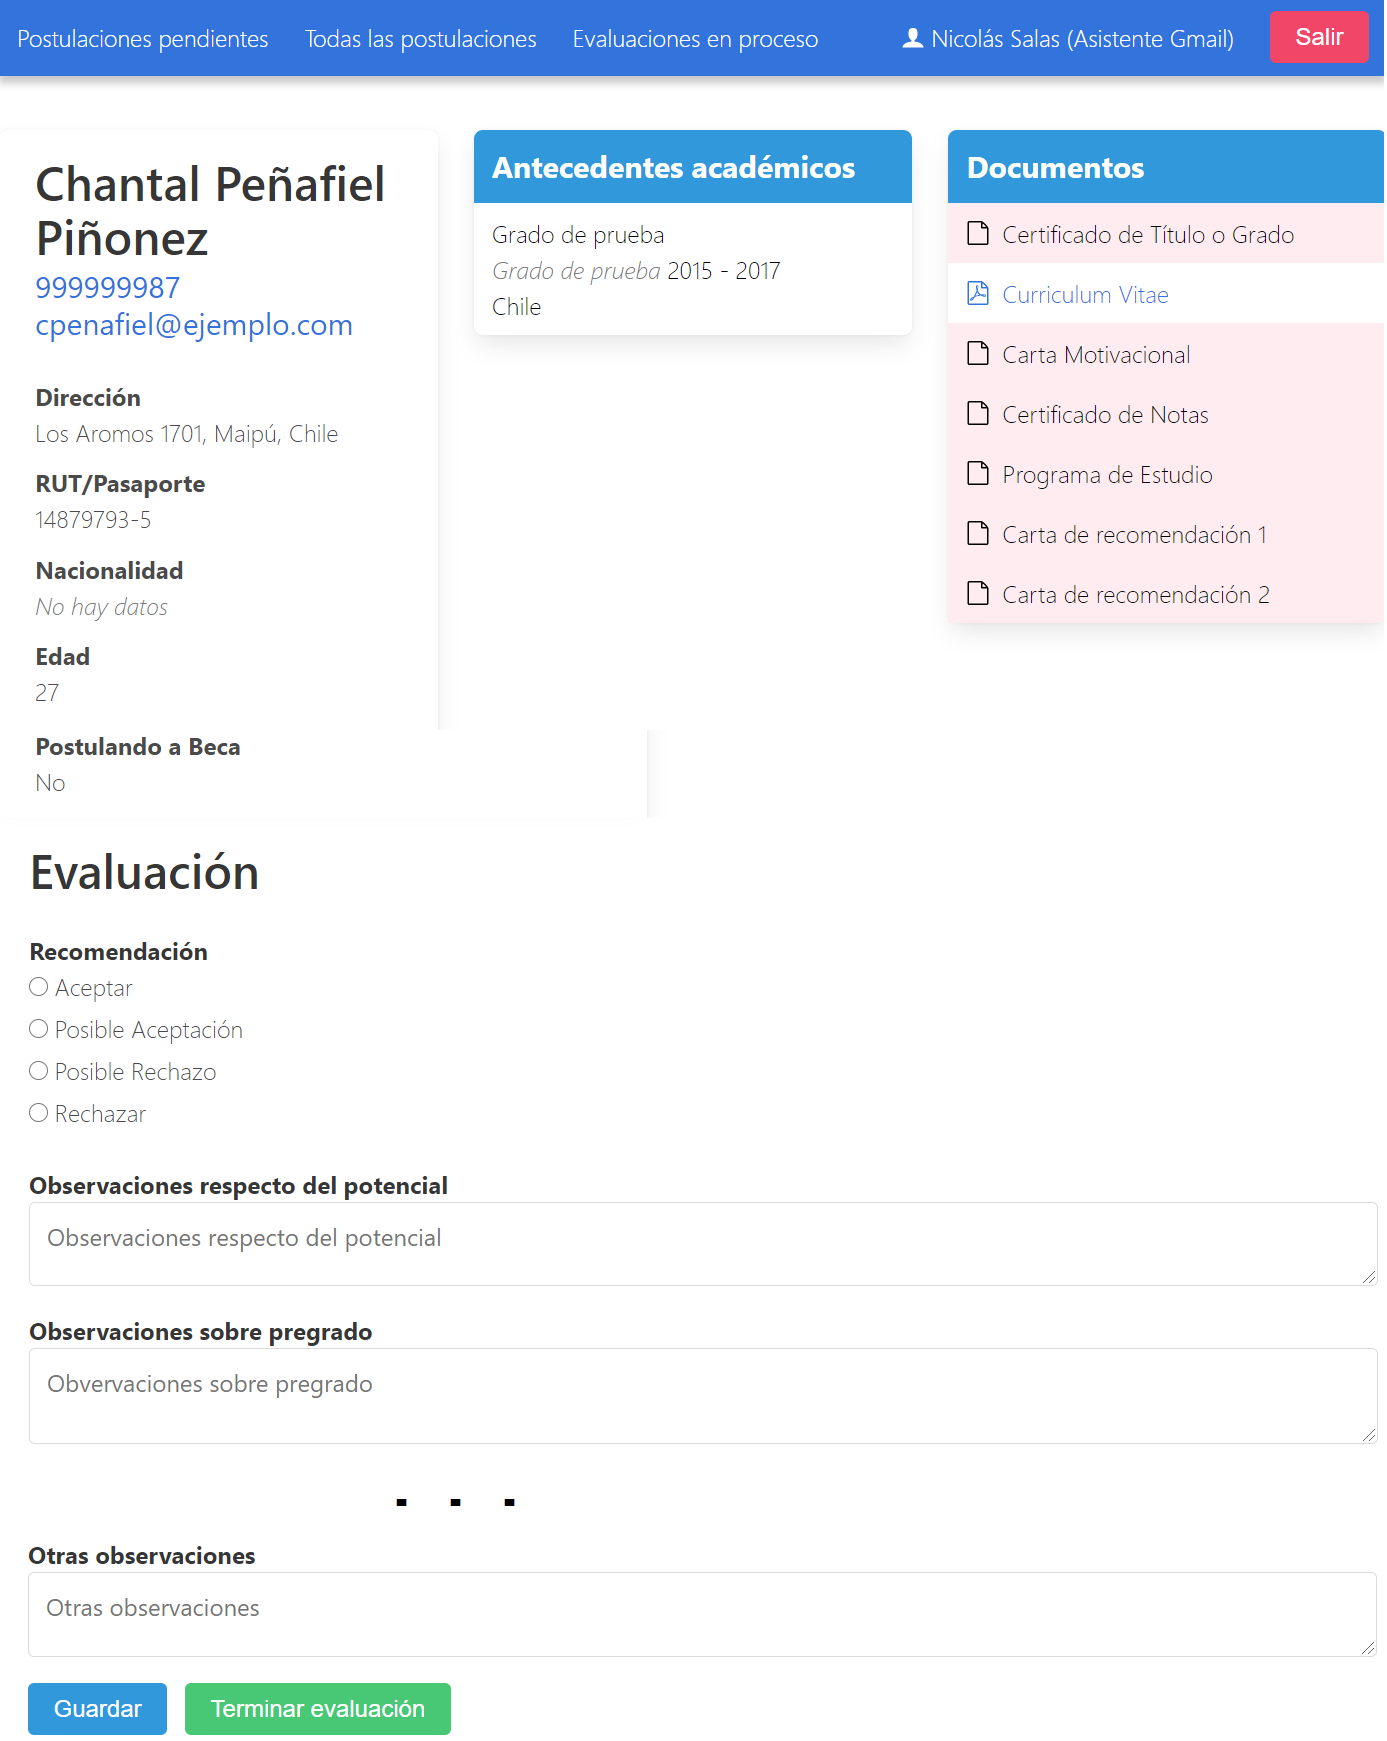
\includegraphics[scale=0.33]{imagenes/04-formulario-evaluacion.png}
    \end{center}
    \caption{Formulario de evaluación de una postulación}
    \label{fig:formulario-evaluacion}
\end{figure}

Una cuarta diferencia entre las interfaces de los evaluadores y los asistentes
consiste en que los primeros, una vez que han emitido su opinión, pueden acceder
a las opiniones emitidas por otros miembros del comité académico. Los asistentes
no tienen acceso a los comentarios de los evaluadores.

\subsection{Interfaces de Usuario para el Coordinador}

Al igual que en los casos anteriores, la opción de menú “Postulaciones
pendientes” muestra todas aquellas postulaciones sobre las cuales el coordinador
tiene algo pendiente (una acción que tomar). En la figura
\ref{fig:pendientes-coordinador} se muestran postulaciones en estado “pendiente
de validación”, las cuales corresponden a aquellas que aún no se han mandado a
evaluar. También se muestran las que están“en evaluación por el comité
académico”, y finalmente, aquellas que están esperando una resolución por parte
del usuario coordinador.

\begin{figure}[!ht]
    \begin{center}
        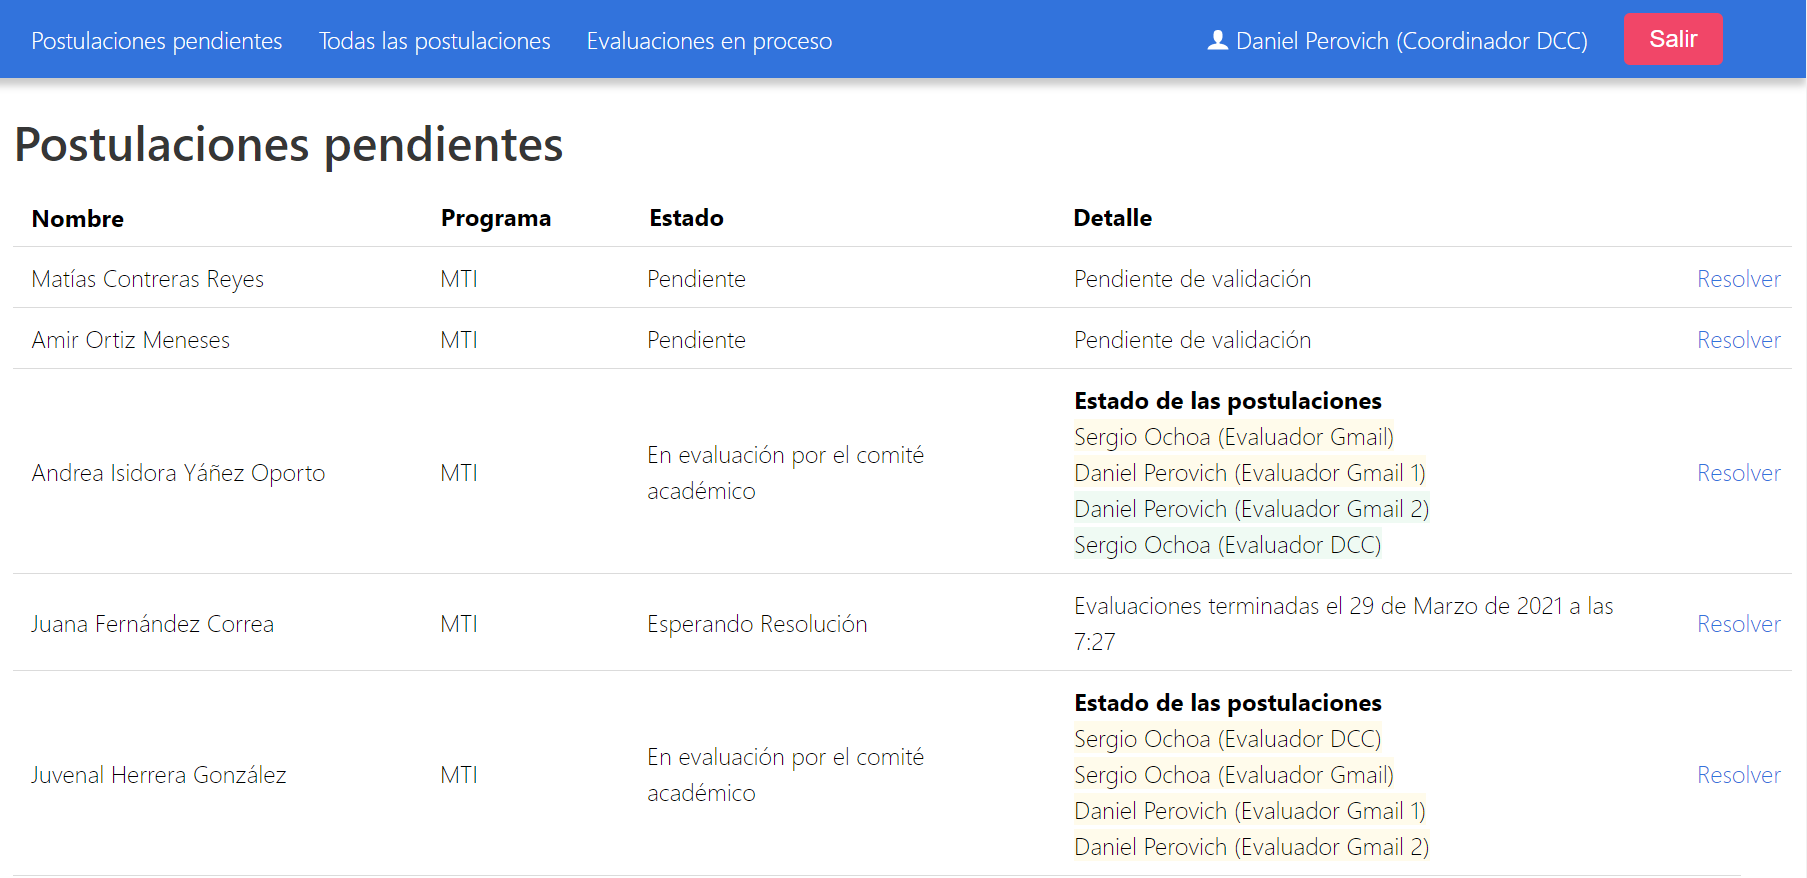
\includegraphics[scale=0.23]{imagenes/04-pendientes-coordinador.png}
    \end{center}
    \caption{Postulaciones pendientes para un usuario coordinador}
    \label{fig:pendientes-coordinador}
\end{figure}

Una vez que una postulación cuenta con la opinión de tres o más evaluadores, el
coordinador puede acceder y resolver sobre la aceptación o rechazo del
postulante. En la Figura \ref{fig:pendientes-coordinador}, la cuarta postulación
se encuentra en ese estado. Para tomar una decisión el coordinador clickear en
“Resolver” y accede al formulario que se muestra en la Figura
\ref{fig:resolucion} (vista parcial del formulario real).

\begin{figure}[!ht]
    \begin{center}
        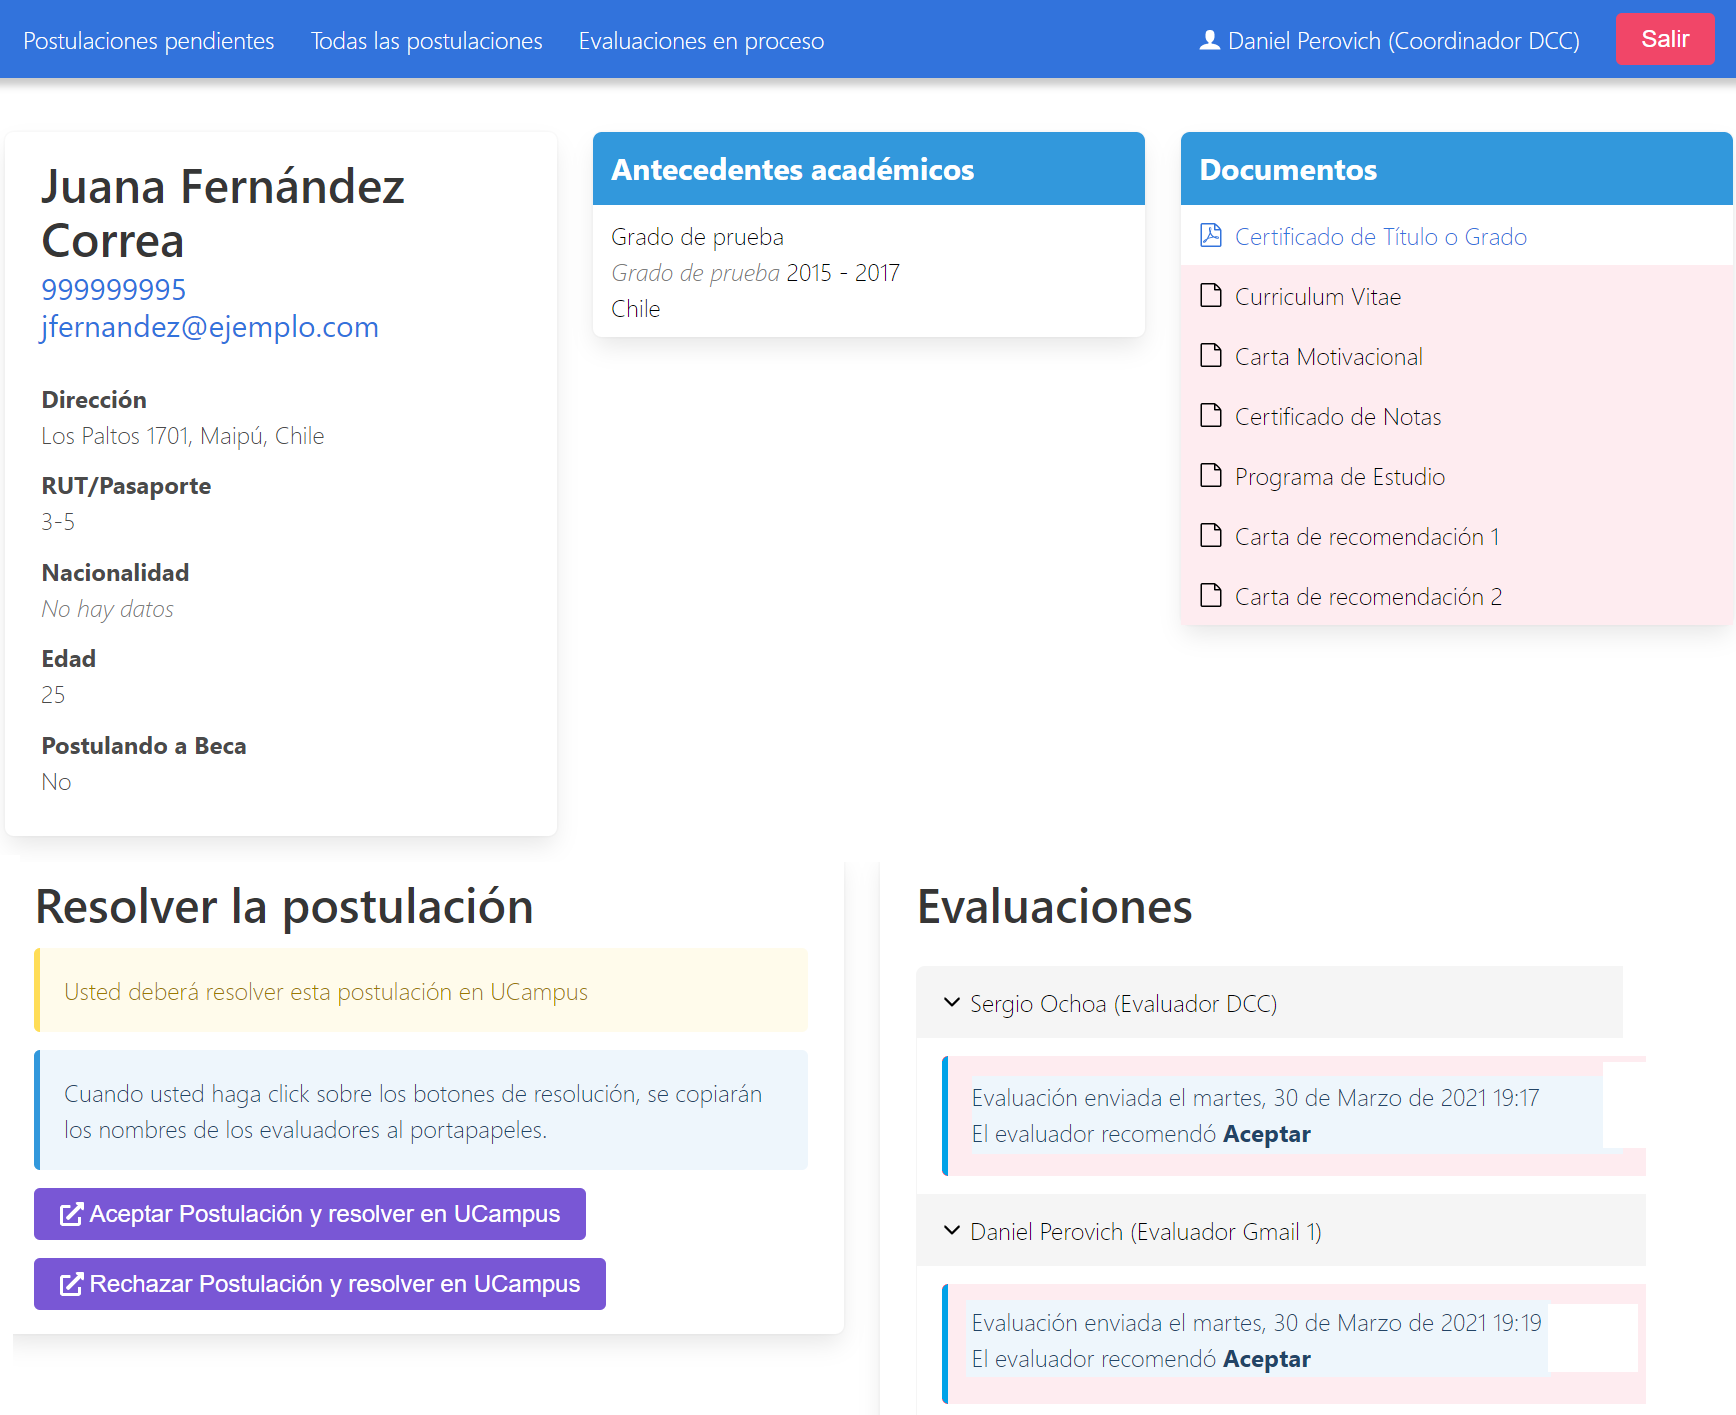
\includegraphics[scale=0.23]{imagenes/04-resolucion.png}
    \end{center}
    \caption{Formulario de resolución de postulaciones}
    \label{fig:resolucion}
\end{figure}

Para terminar, una vez que el coordinador emite su evaluación sobre el
postulante, la postulación avanza al estado “Esperando Resolución”. En este
estado, el coordinador debe resolver si acepta o rechaza la postulación. Para
ello, la figura \ref{fig:resolucion} muestra dos botones en el lado izquierdo de
la interfaz, uno para aceptar y otro para rechazar la postulación. Al lado
derecho en dicha interfaz se muestran las evaluaciones y recomendaciones de cada
evaluador.

Sea cual sea la decisión del coordinador, en el momento en que se presiona
cualquiera de los botones, se termina el proceso interno de evaluación de una
postulación, y ésta debe resolverse en UCampus. Esto es porque a pesar de que el
sistema marque la postulación como resuelta, UCampus no expone una forma de
resolver postulaciones, y por dicha razón, se debe resolver la postulación
dentro de UCampus.

Mientras tanto, el sistema internamente marca la postulación como resuelta.
Cuando una postulación ya está resuelta internamente en el sistema de evaluación
de postulaciones, el coordinador verá la interfaz mostrada en la figura
\ref{fig:postulacion-resuelta}, la que le permite (en caso de ser necesario)
devolver la postulación al estado “Esperando Resolución”. Esto se hace
clickeando el botón “Volver a evaluación”. La razón de esta interfaz es para
poder mitigar posibles equivocaciones del coordinador, al momento de presionar
los botones que indican la aceptación o rechazo de una postulación.

\begin{figure}[!ht]
    \begin{center}
        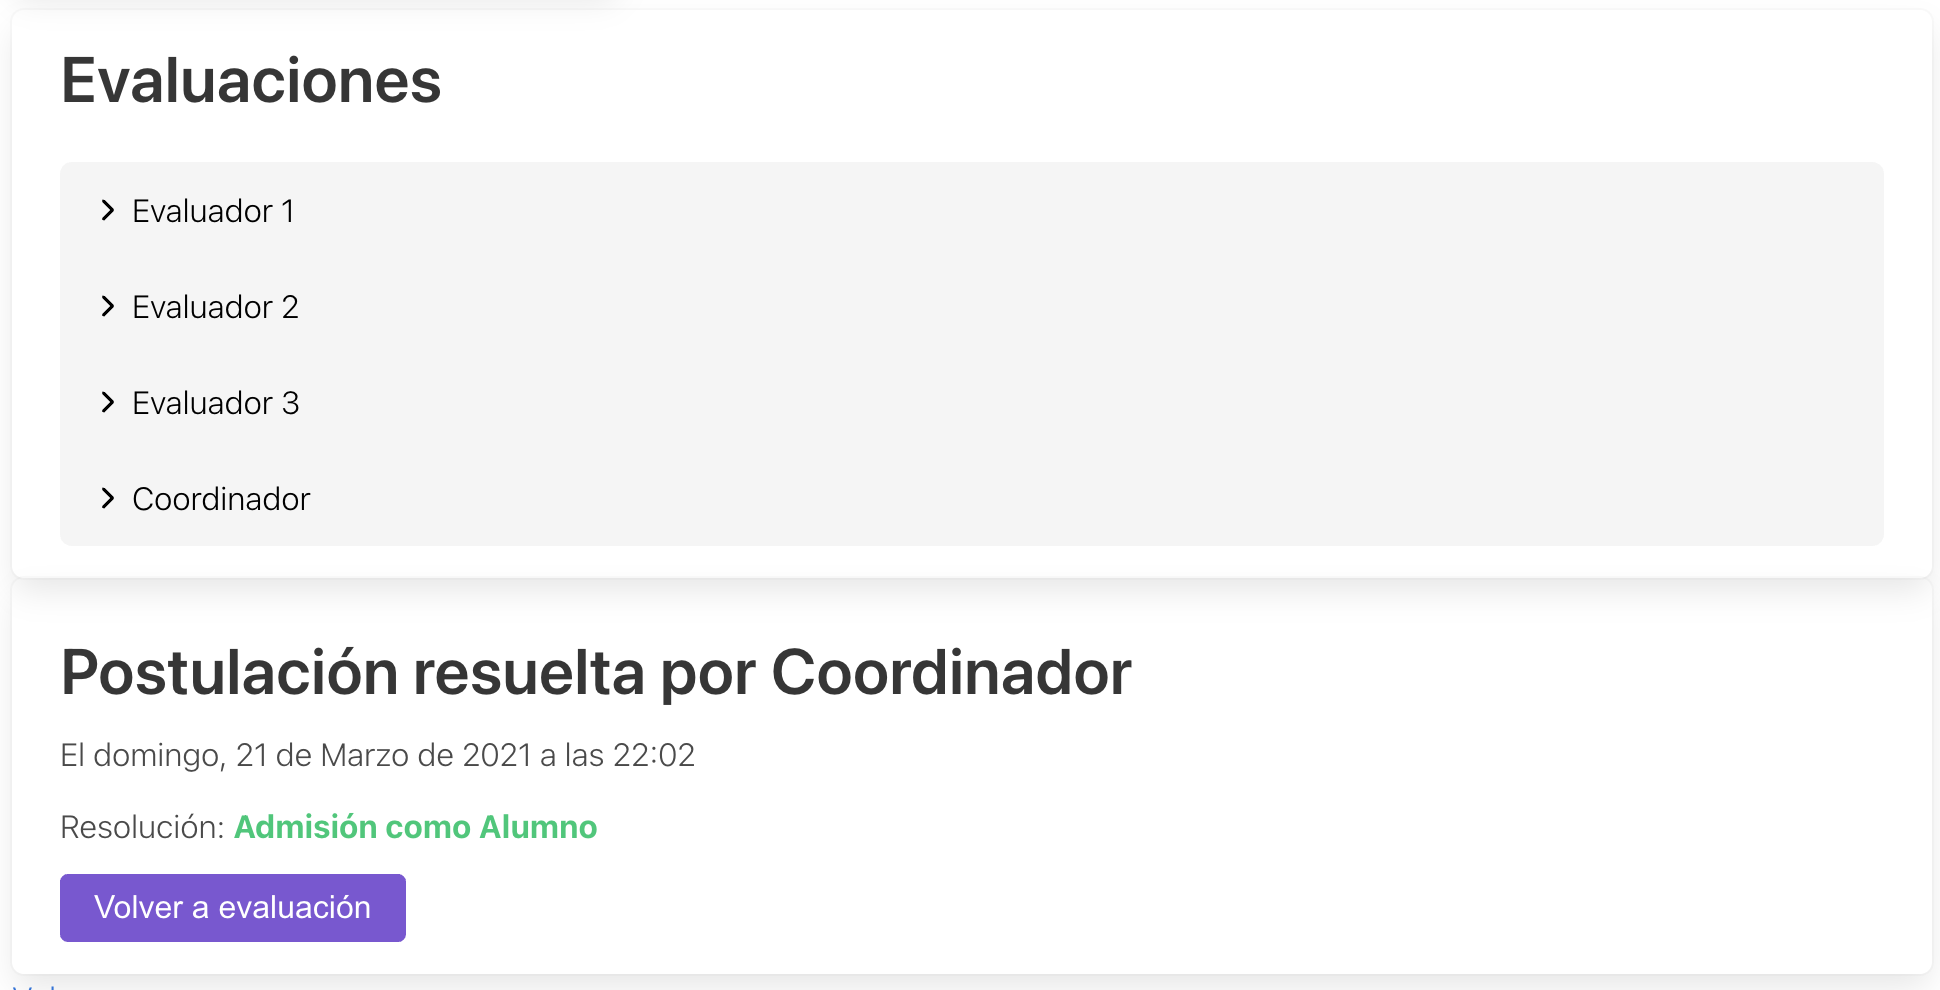
\includegraphics[scale=0.44]{imagenes/04-postulacion-resuelta.png}
    \end{center}
    \caption{Interfaz para el coordinador de una postulación resuelta}
    \label{fig:postulacion-resuelta}
\end{figure}